\documentclass[tikz,border=5pt]{standalone}
\usepackage{amsmath}
\usepackage{pgfplots}
\pgfplotsset{compat=1.18}

\definecolor{corba}{HTML}{365FB3}
\definecolor{punt}{HTML}{B91C1C}

\begin{document}
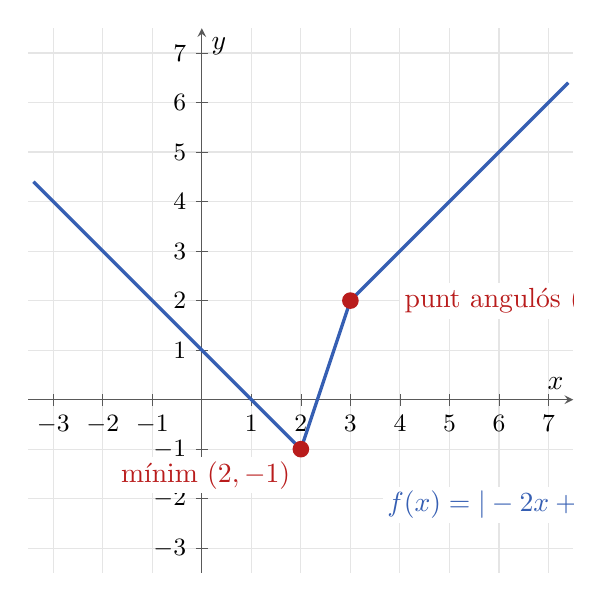
\begin{tikzpicture}
  \begin{axis}[
    width=11.5cm,
    height=8.5cm,
    axis lines=middle,
    xmin=-3.5,
    xmax=7.5,
    ymin=-3.5,
    ymax=7.5,
    xlabel={$x$},
    ylabel={$y$},
    xtick={-3,-2,-1,0,1,2,3,4,5,6,7},
    ytick={-3,-2,-1,0,1,2,3,4,5,6,7},
    grid=major,
    grid style={black!10},
    axis line style={black!65},
    tick style={black!65},
    tick label style={font=\small},
    unit vector ratio*=1 1 1,
    clip=true,
  ]
    \addplot[corba, very thick, domain=-3.4:2, samples=2] {-x+1};
    \addplot[corba, very thick, domain=2:3, samples=2] {3*x-7};
    \addplot[corba, very thick, domain=3:7.4, samples=2] {x-1};

    \addplot[only marks, mark=*, mark size=2.8pt, punt]
      coordinates {(2,-1) (3,2)};

    \node[anchor=north east, text=punt, fill=white, inner sep=1.5pt]
      at (axis cs:1.88,-1.15) {m\'inim $(2,-1)$};
    \node[anchor=west, text=punt, fill=white, inner sep=1.5pt]
      at (axis cs:4,2) {punt angul\'os $(3,2)$};
    \node[anchor=south west, text=corba, fill=white, inner sep=1.5pt]
      at (axis cs:3.65,-2.5) {$f(x)=|-2x+4|-|x-3|$};
  \end{axis}
\end{tikzpicture}
\end{document}
